\chapter{Training with signal events and results}
\label{chap:RESULTS}

After the optimization of the weight clipping parameter, it is possible to train the network with signal events in the observed dataset. Obviously, the operation has to be done with $W$ set to the value found for the corresponding reference dataset size. In this case the output of the algorithm will be the distribution of $t$ obsereved when there are new physics signals in the data. This result can be translated into a median significance, which must be compared with the ideal significance. The computation of this ideal test value is done in the next Section. Then, the results of this new phase of network training are presented.





\section{Ideal significance computation}
In the following discussion, the variable $x$ will be identified with the invariant mass. In fact, we are able to evaluate the ideal log-likelihood ratio with a monodimensional distribution after fitting it.

What we have is a histogram of $M_Z$ and its bins can be used as points to fit. However, it is not convenient to fit the whole spectrum because it is expected that the distribution of $M_{Z}$ in the reference and in the alternative hypoteses are the same except for an interval where they differ. So the log-likelihood ratio is different from 0 only in this interval, that must be defined for both \textbf{Zprime-Zmumu} and \textbf{EFT\_YW06} datasets as well as the functions used to fit. The procedure adopted is the following:

\begin{itemize}
	\item For the \textbf{Zmumu-Zprime} dataset, the reference distribution differs from the one with new physics signals only in the interval $[250,350]~\si{GeV/c^2}$. In this region the background distribution is approximated by a power law:
	\begin{equation}
		n_\mathrm{bkg}(x) = a\operatorname{e}^{bx + c} + d
	\end{equation}
	while the signal distribution is described by the sum of two gaussians:
	\begin{equation}
		n_\mathrm{sig}(x) = a\exp{\left[-\frac{(x-b)^2}{c^2}\right]} 
		+ d\exp{\left[-\frac{(x-e)^2}{f^2}\right]}
	\end{equation}
	When fitting the signal+background distribution, $n_\mathrm{bkg}$ and $n_\mathrm{sig}$ should be summed and then normalized.
	
	\item For the \textbf{EFT\_YW06} dataset, the distribution with new physics events is similar to the reference one, but with a different slope in the exponential descent. An interval sufficiently populated where they differ is $[200,800]~\si{GeV/c^2}$. In this region both distributions are approximated by a power law with a linear growth:
	\begin{align}
		n_\mathrm{bkg}(x) &= a_{1}x\operatorname{e}^{b_{1}x + c_{1}} + d_{1}	\\
		n_\mathrm{sig+bkg}(x) &= a_{2}x\operatorname{e}^{b_{2}x + c_{2}} + d_{2}
	\end{align}
\end{itemize}

Now that good approximants of the distributions are known, we can compute the log-likelihood ratio of $n_\mathrm{bkg+sig}$ and $n_\mathrm{bkg}$ by integration of the the funtion log-ratio of the two distributions. The ideal significance is then calculated through the Equation \ref{eqn:ID_SIG}. In Figure \ref{fig:ID_SIG_ZMUMU_ZPRIME} a schematization of this procedure is given as an example.

\begin{figure}[H]
	\centering
	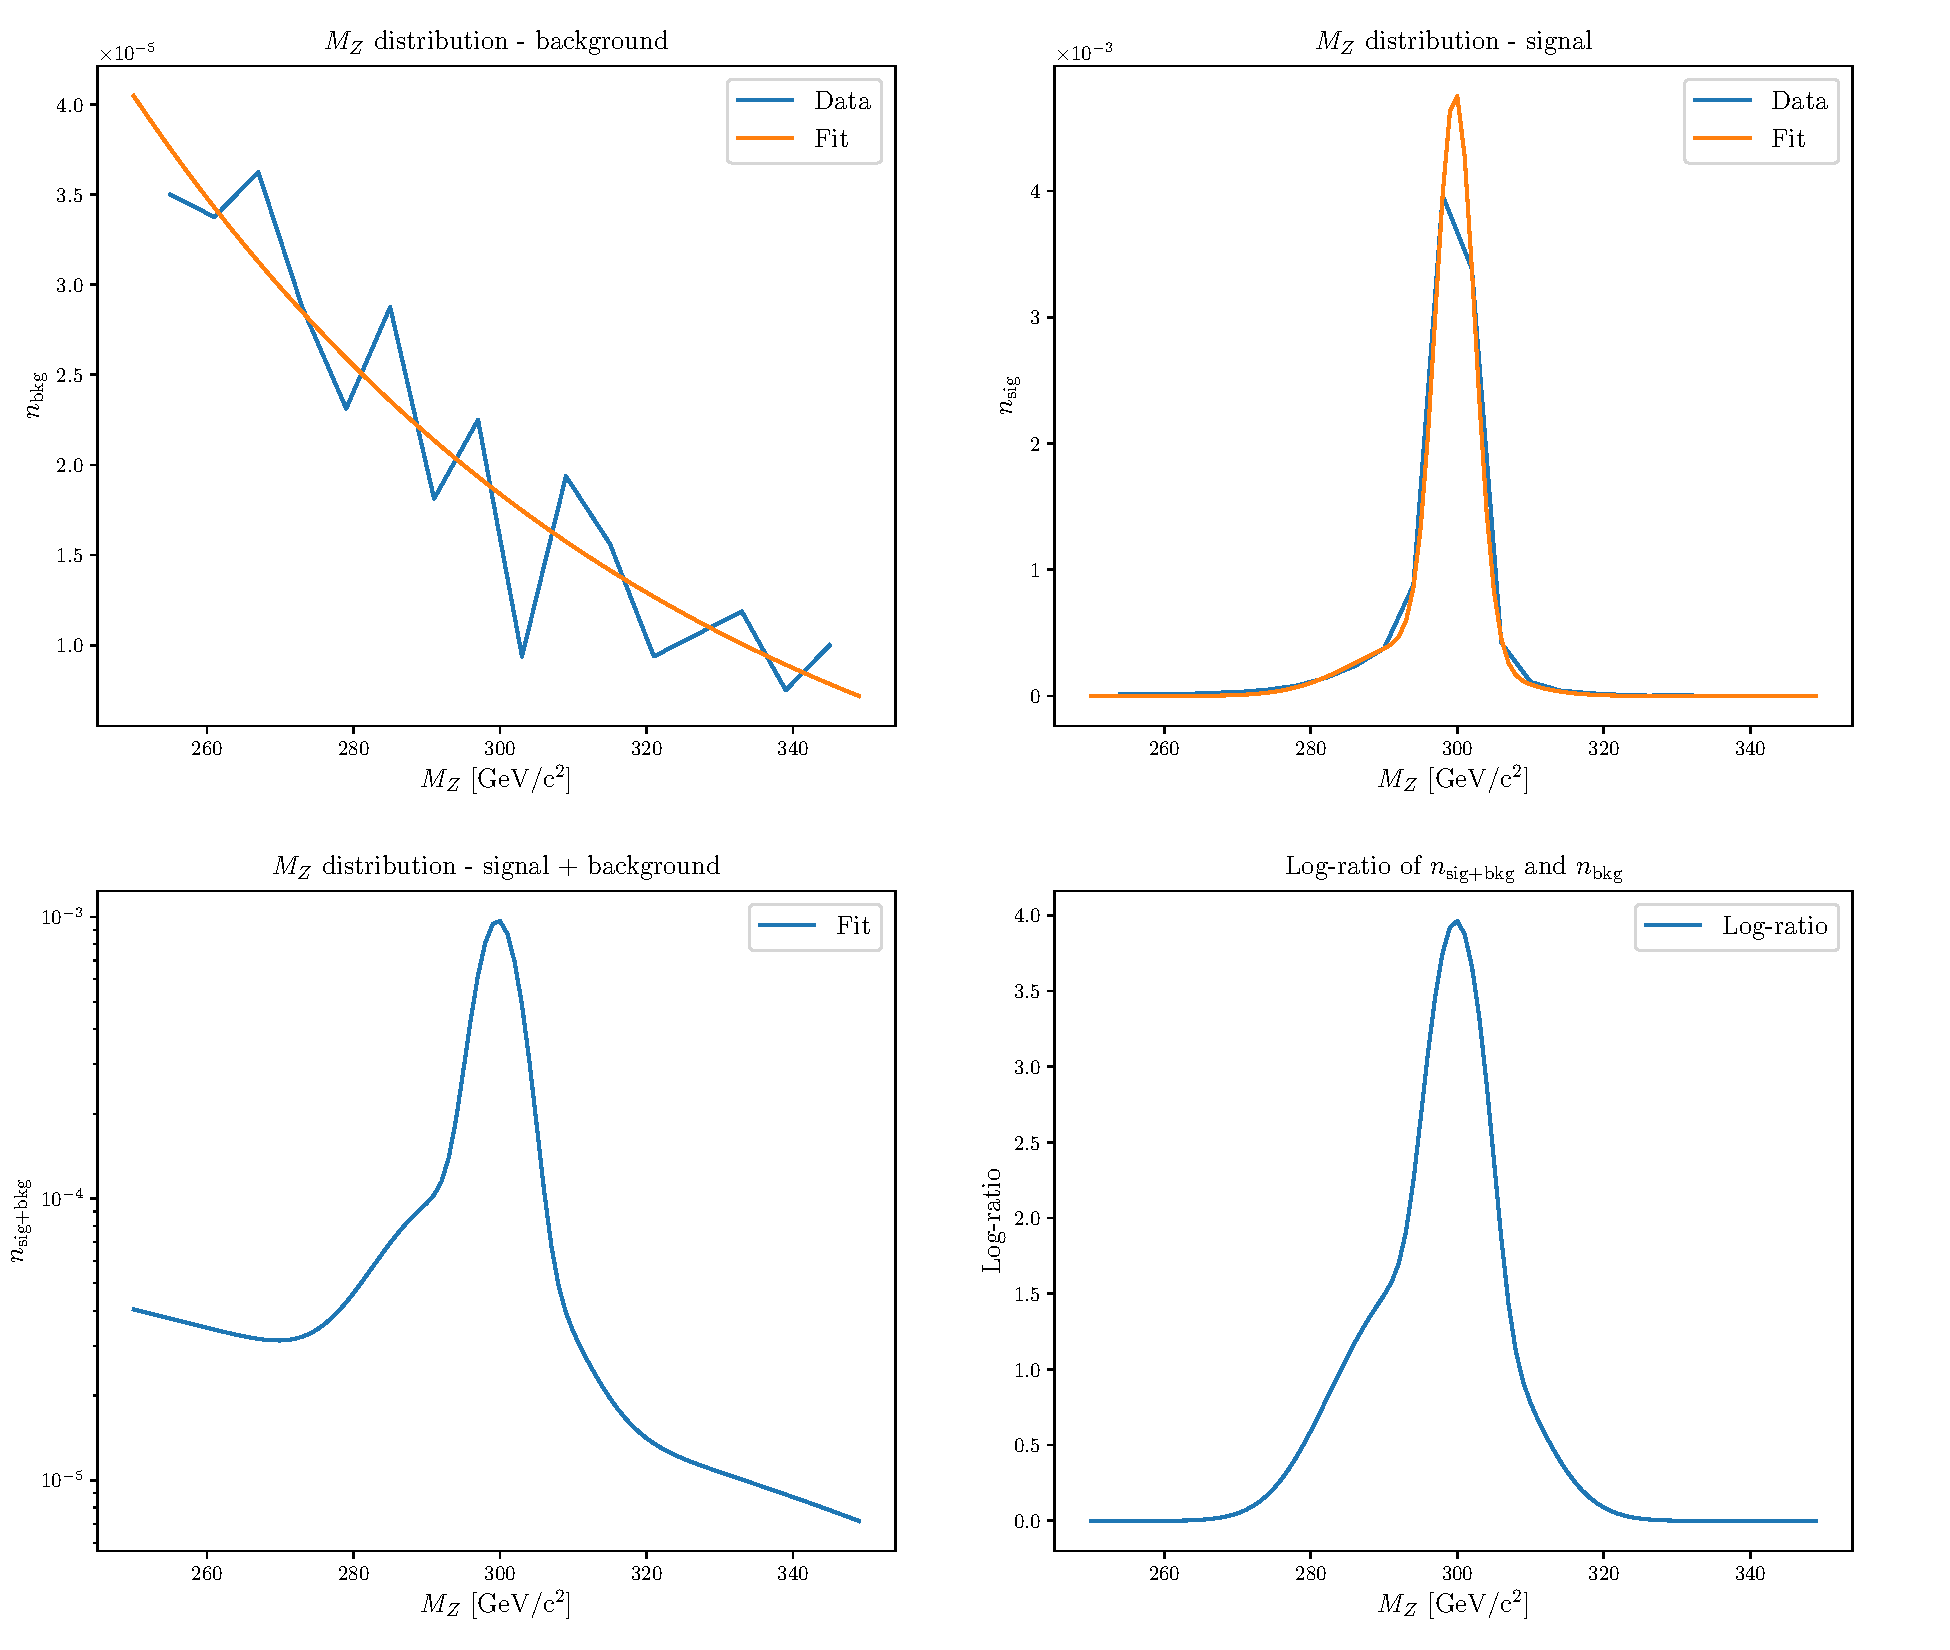
\includegraphics[width=1.0\textwidth]{Python/RESULTS/ID_SIG/id_sig_Zmumu_Zprime.pdf}
	\caption{Ideal significance computing. Top row: background and signal distributions with their fit in the interval $[250,350]~\si{GeV/c^2}$. Bottom row: signal+background distribution and log-ratio of $n_\mathrm{bkg+sig}$ and $n_\mathrm{bkg}$.}
	\label{fig:ID_SIG_ZMUMU_ZPRIME}
\end{figure}

Finally, the results for ideal significance calculation are listed below:
\begin{align*}
	\textbf{Zmumu-Zprime}	&	\qquad	\sigma_\mathrm{id} \approx 11,8\sigma	\\
	\textbf{EFT\_YW06}		&	\qquad	\sigma_\mathrm{id} \approx 25\sigma		
\end{align*}





\section{Training results: $t_\mathrm{obs}$ distribution and observed significance}
The results of training processes for both \textbf{Zmumu-Zprime} and \textbf{EFT\_YW06} datasets and for the several sizes of the reference are presented in this Section. The relevant informations showed are the $t_\mathrm{obs}$ distribution and the quantile plot, which tells us if the process of training gives a stable $t_\mathrm{obs}$ distribution after a certain number of epochs. The value of the observed significance, reported in the plots, is obtained through:
\begin{equation}
	\sigma_\mathrm{obs} = \sqrt{2} * \operatorname{erf^{-1}}(1-p_\mathrm{obs})
\end{equation}
where $p$ is the median $p$-value computed through the median $t$ of the observed distribution, denoted as $t_\mathrm{obs}$:
\begin{equation}
	p_\mathrm{obs} = \int_{-\infty}^{t_\mathrm{med}} \chi^2(t;\nu=96) \d t
\end{equation}


\subsection*{Zmumu-Zprime dataset}
\vspace{-5mm}
\begin{figure}[H]
	\centering
	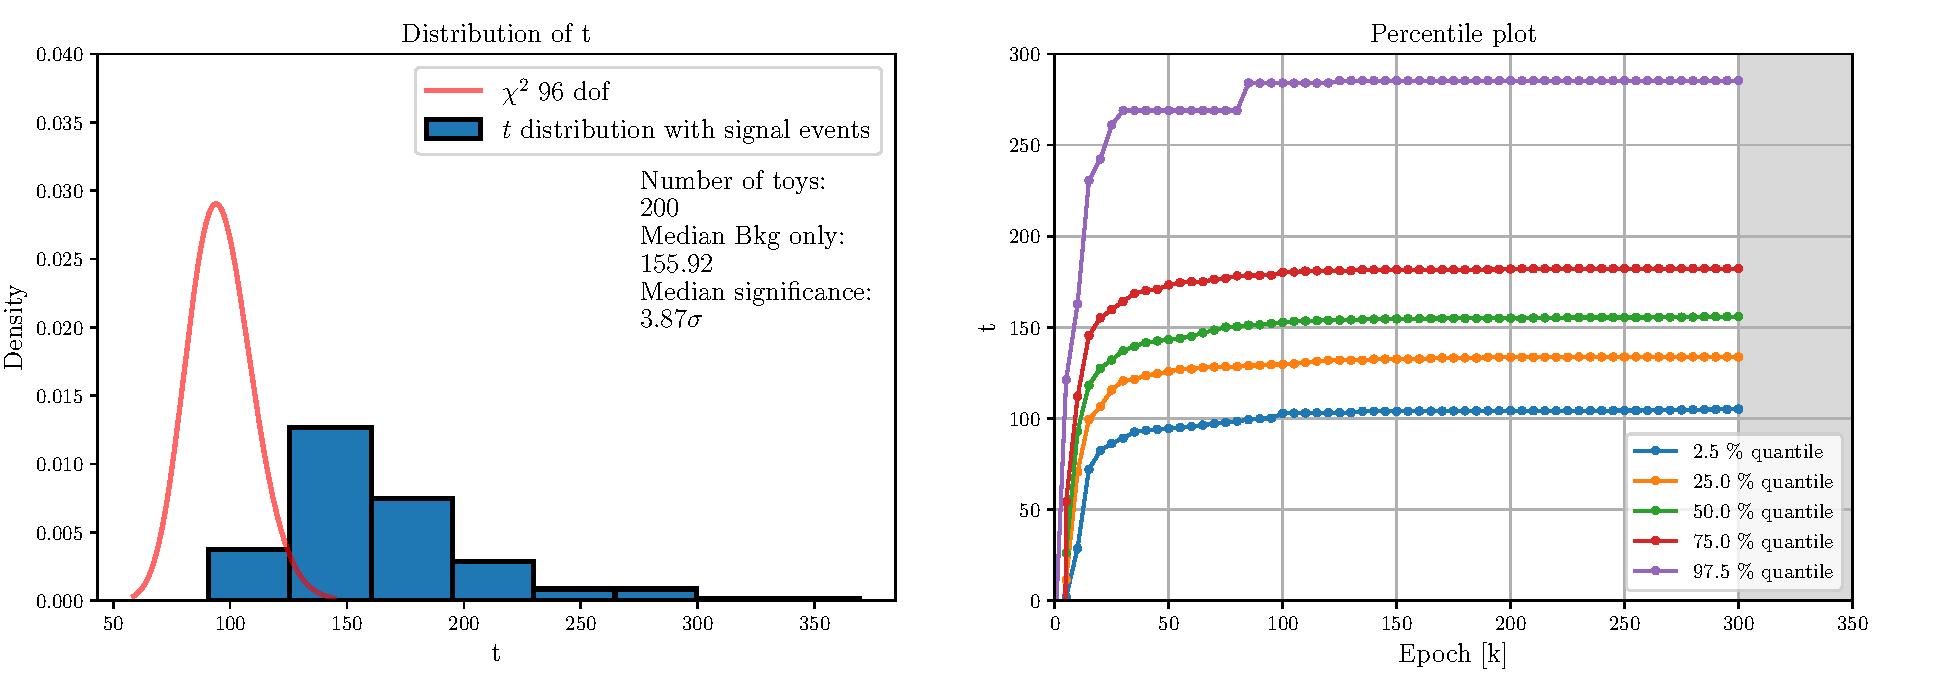
\includegraphics[width=1.0\textwidth]{Python/RESULTS/ref100000_bkg20000_sig40/data_ref100000_bkg20000_sig40_wclip2-15.pdf}
	\caption{Results for $N_\mathrm{ref}=100\si{k}$, $N_\mathrm{bkg}=20\si{k}$, $N_\mathrm{sig}=40$, $W=2.15$.}
	\label{fig:REF100000_BKG20000_SIG40_WCLIP2.15}
\end{figure}
\vspace{-5mm}
\begin{figure}[H]
	\centering
	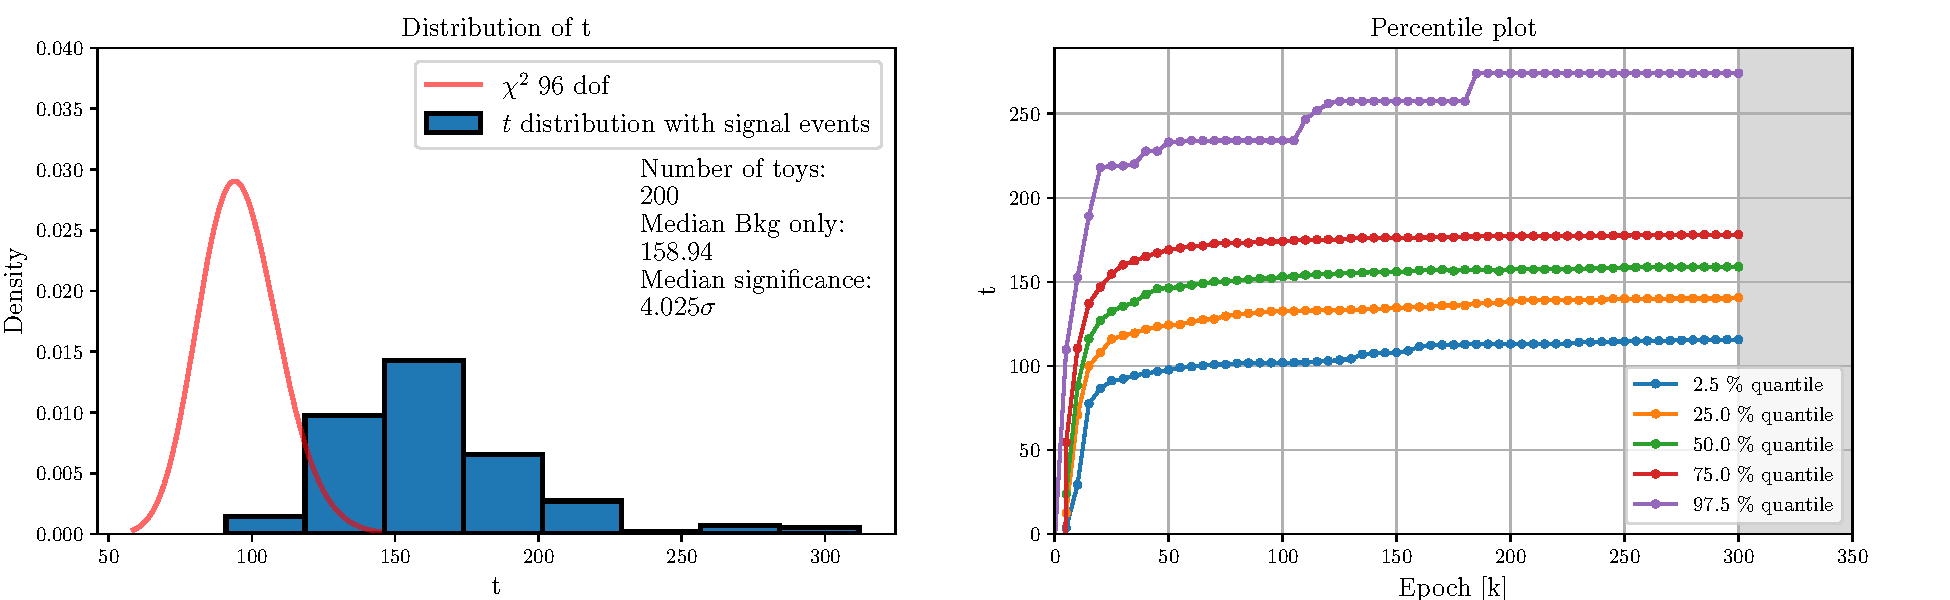
\includegraphics[width=1.0\textwidth]{Python/RESULTS/ref200000_bkg20000_sig40/data_ref200000_bkg20000_sig40_wclip2-4.pdf}
	\caption{Results for $N_\mathrm{ref}=200\si{k}$, $N_\mathrm{bkg}=20\si{k}$, $N_\mathrm{sig}=40$, $W=2.4$.}
	\label{fig:REF200000_BKG20000_SIG40_WCLIP2.4}
\end{figure}
\vspace{-5mm}
\begin{figure}[H]
	\centering
	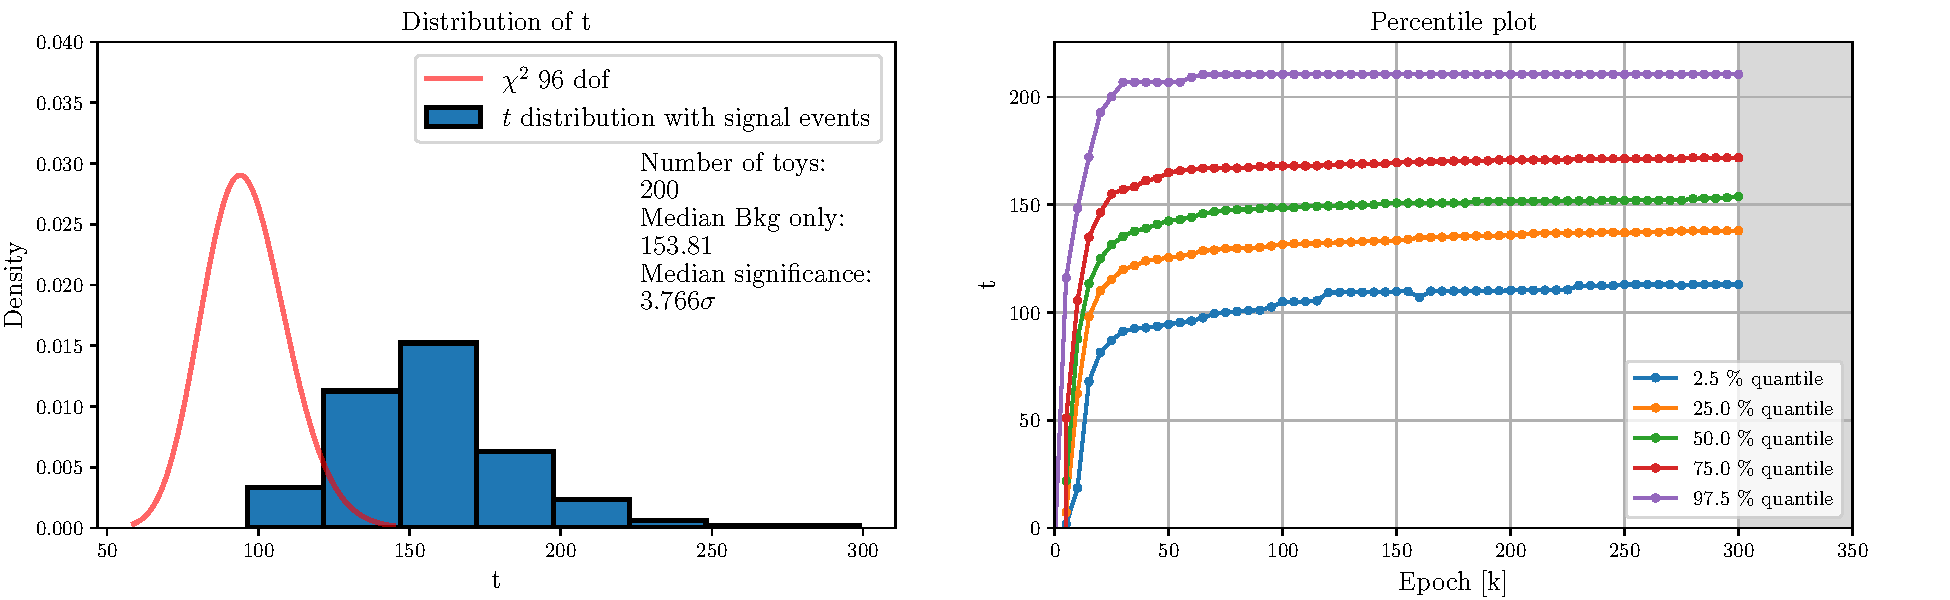
\includegraphics[width=1.0\textwidth]{Python/RESULTS/ref300000_bkg20000_sig40/data_ref300000_bkg20000_sig40_wclip2-45.pdf}
	\caption{Results for $N_\mathrm{ref}=300\si{k}$, $N_\mathrm{bkg}=20\si{k}$, $N_\mathrm{sig}=40$, $W=2.45$.}
	\label{fig:REF300000_BKG20000_SIG40_WCLIP2.45}
\end{figure}
\vspace{-5mm}
\begin{figure}[H]
	\centering
	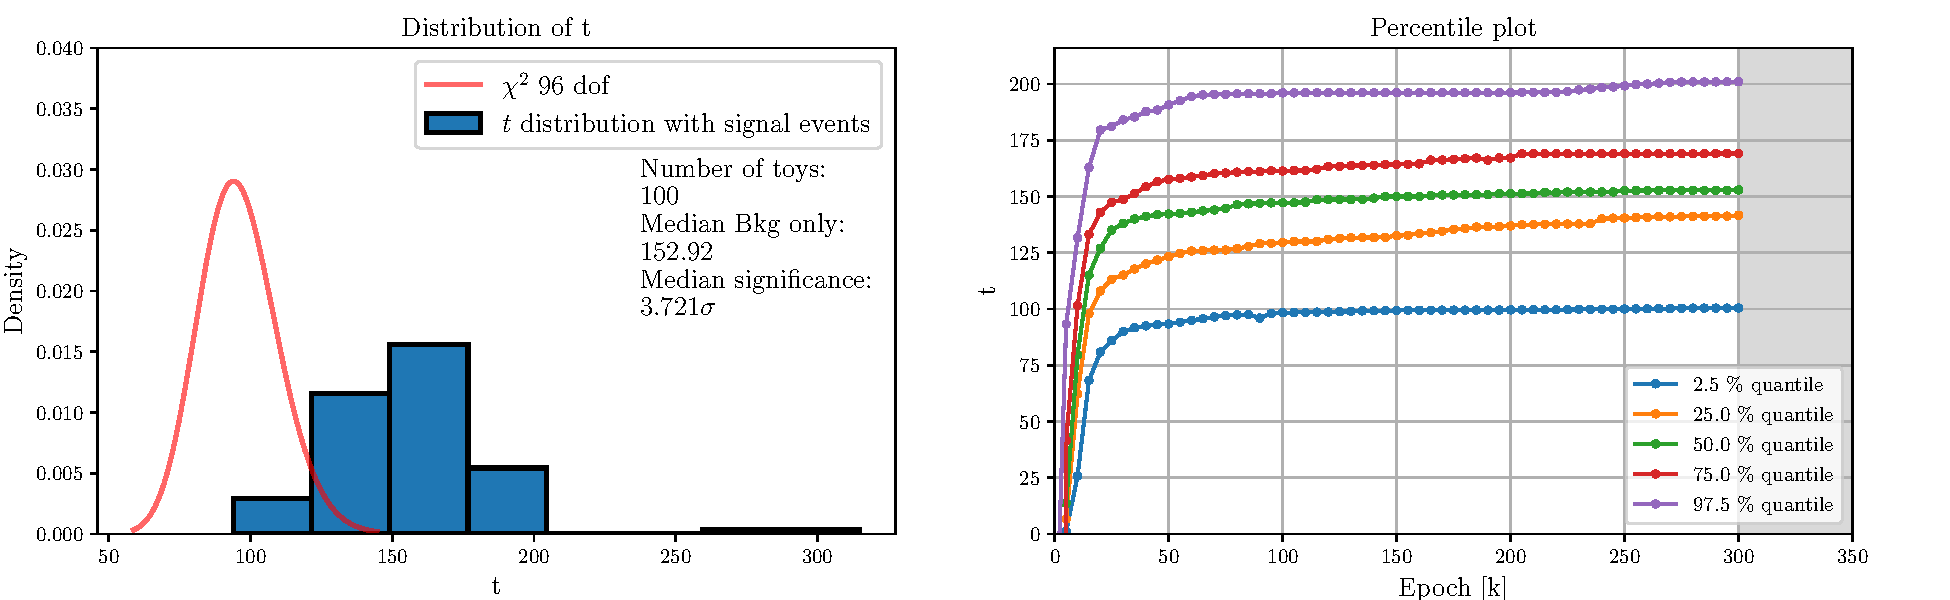
\includegraphics[width=1.0\textwidth]{Python/RESULTS/ref500000_bkg20000_sig40/data_ref500000_bkg20000_sig40_wclip2-55.pdf}
	\caption{Results for $N_\mathrm{ref}=500\si{k}$, $N_\mathrm{bkg}=20\si{k}$, $N_\mathrm{sig}=40$, $W=2.55$.}
	\label{fig:REF500000_BKG20000_SIG40_WCLIP2.55}
\end{figure}
\vspace{-5mm}
\begin{figure}[H]
	\centering
	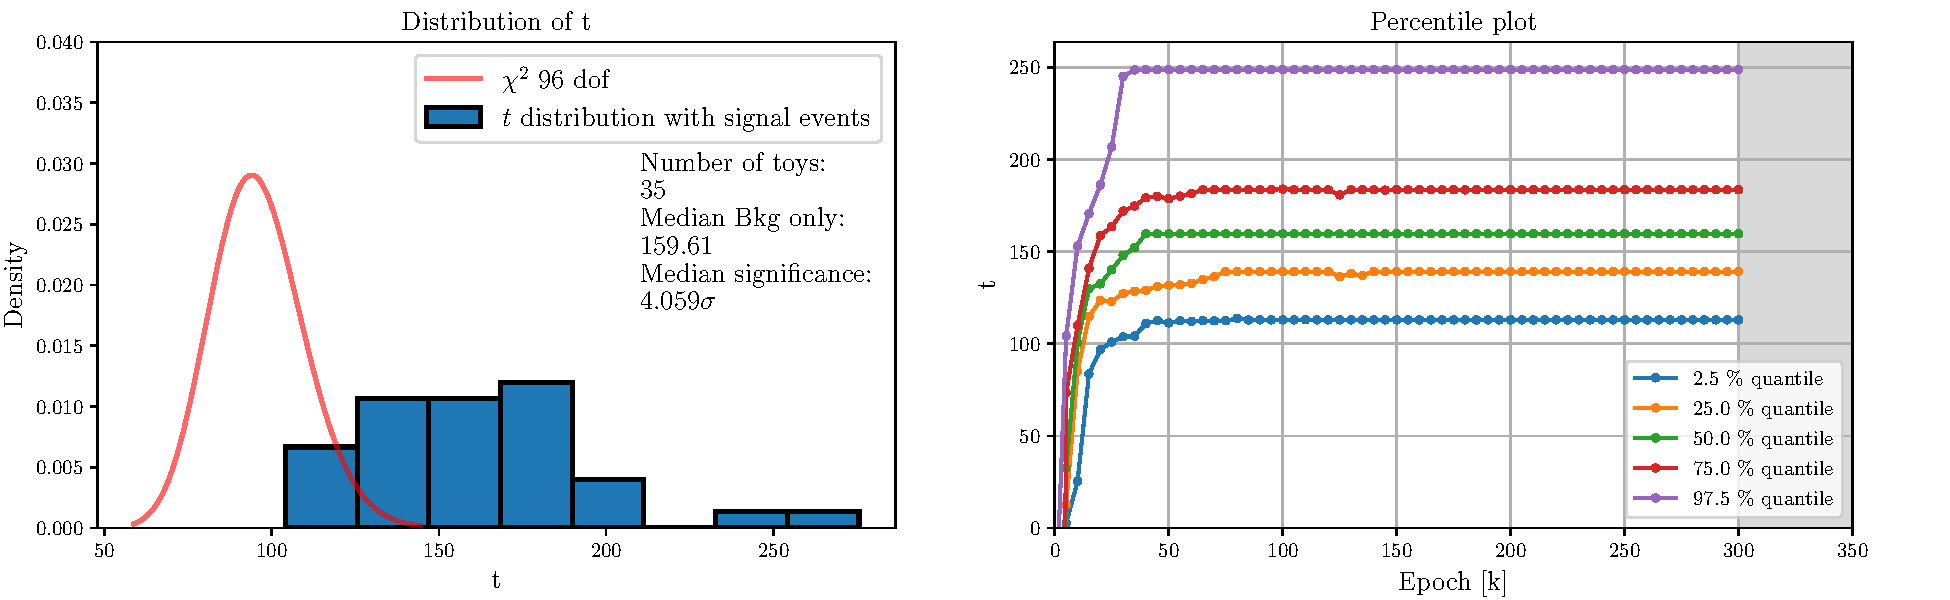
\includegraphics[width=1.0\textwidth]{Python/RESULTS/ref1000000_bkg20000_sig40/data_ref1000000_bkg20000_sig40_wclip2-7.pdf}
	\caption{Results for $N_\mathrm{ref}=1000\si{k}$, $N_\mathrm{bkg}=20\si{k}$, $N_\mathrm{sig}=40$, $W=2.7$.}
	\label{fig:REF1000000_BKG20000_SIG40_WCLIP2.7}
\end{figure}





\subsection*{EFT\_YW06 dataset}
\vspace{-5mm}
\begin{figure}[H]
	\centering
	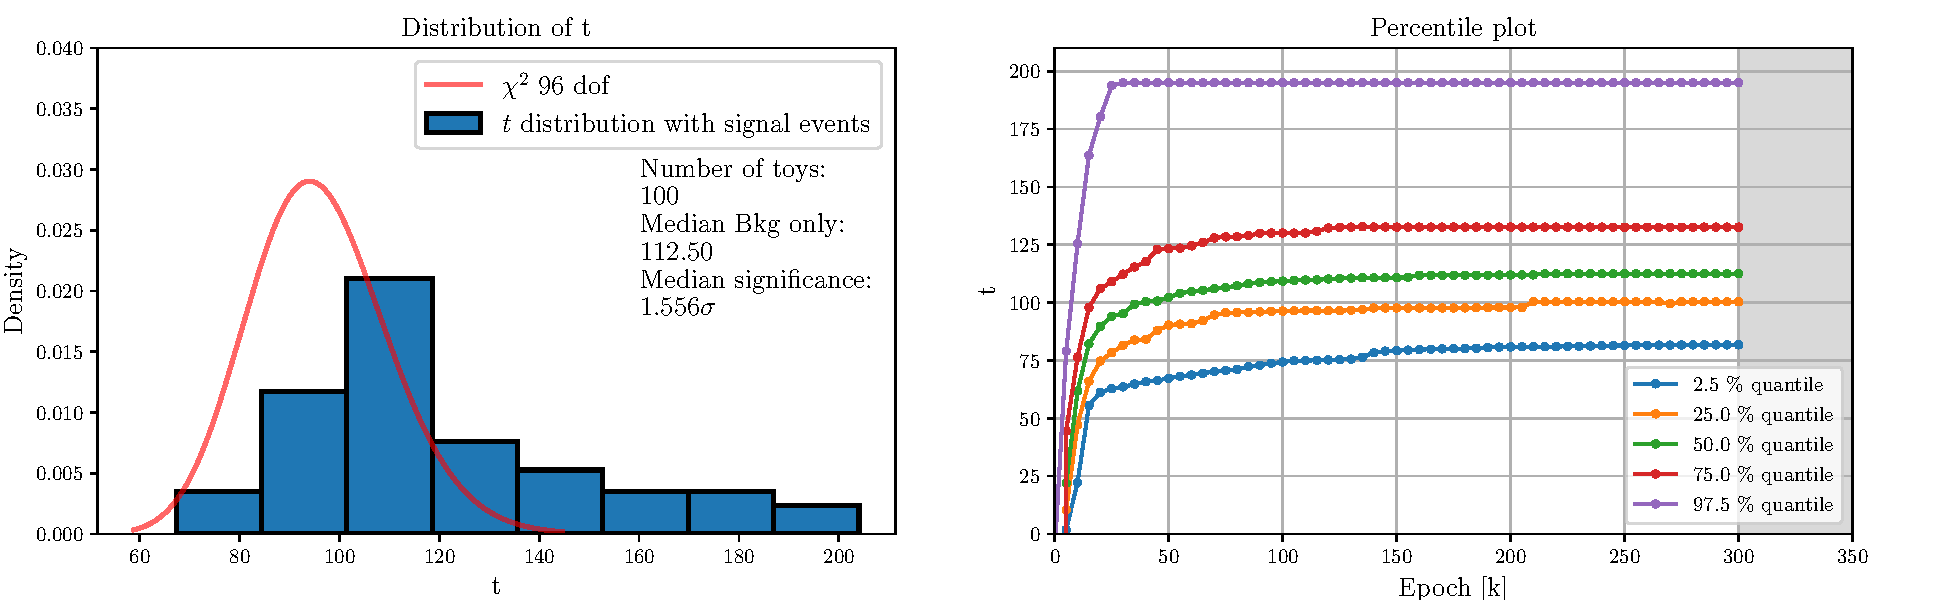
\includegraphics[width=1.0\textwidth]{Python/RESULTS/ref100000_bkg0_eft20000/data_ref100000_bkg0_eft20000_wclip2-25.pdf}
	\caption{Results for $N_\mathrm{ref}=100\si{k}$, $N_\mathrm{eft}=20\si{k}$, $W=2.25$.}
	\label{fig:REF100000_BKG0_EFT20000_WCLIP2.25}
\end{figure}
\vspace{-5mm}
\begin{figure}[H]
	\centering
	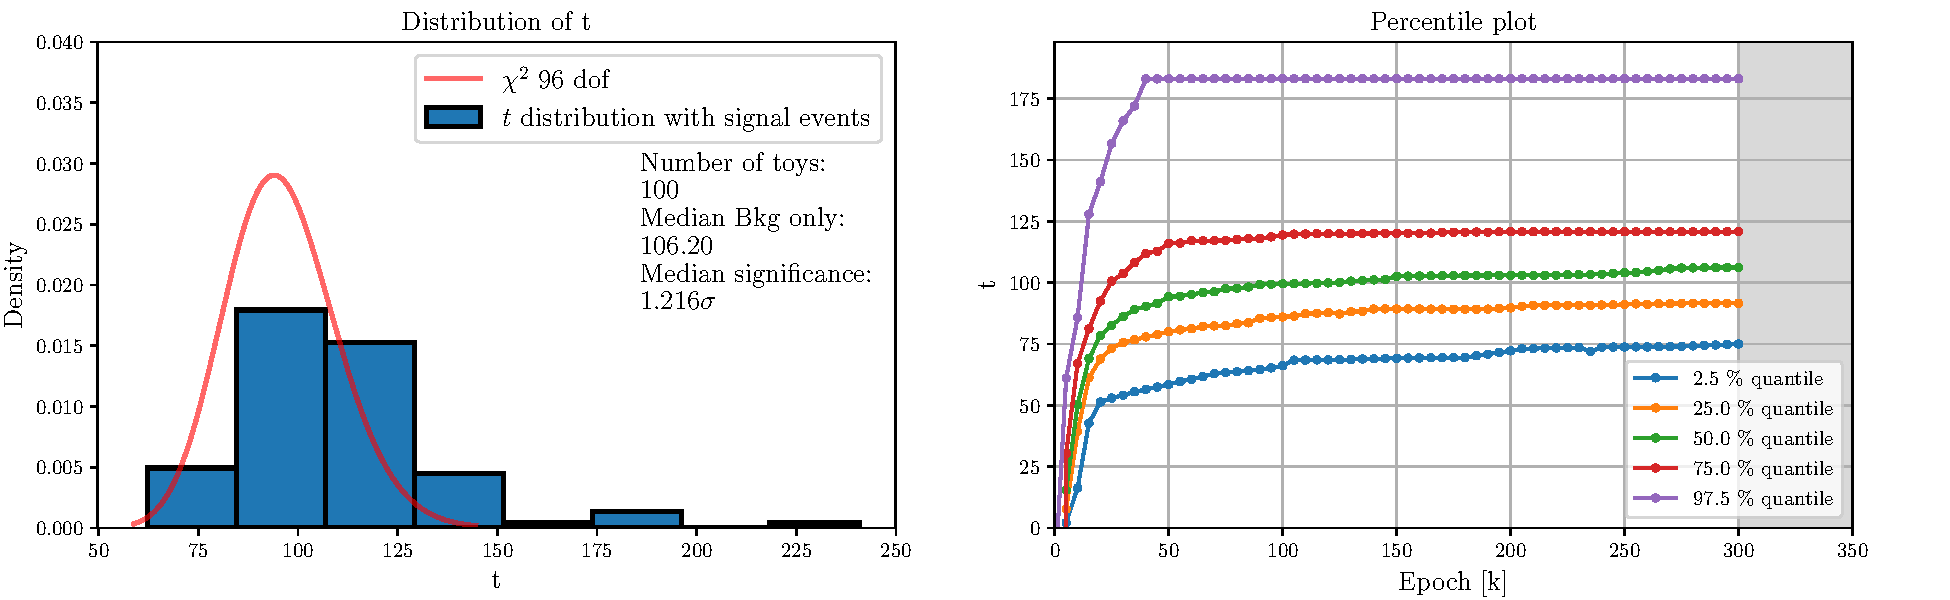
\includegraphics[width=1.0\textwidth]{Python/RESULTS/ref200000_bkg0_eft20000/data_ref200000_bkg0_eft20000_wclip2-4.pdf}
	\caption{Results for $N_\mathrm{ref}=200\si{k}$, $N_\mathrm{eft}=20\si{k}$, $W=2.4$.}
	\label{fig:REF200000_BKG0_EFT20000_WCLIP2.4}
\end{figure}
\vspace{-5mm}
\begin{figure}[H]
	\centering
	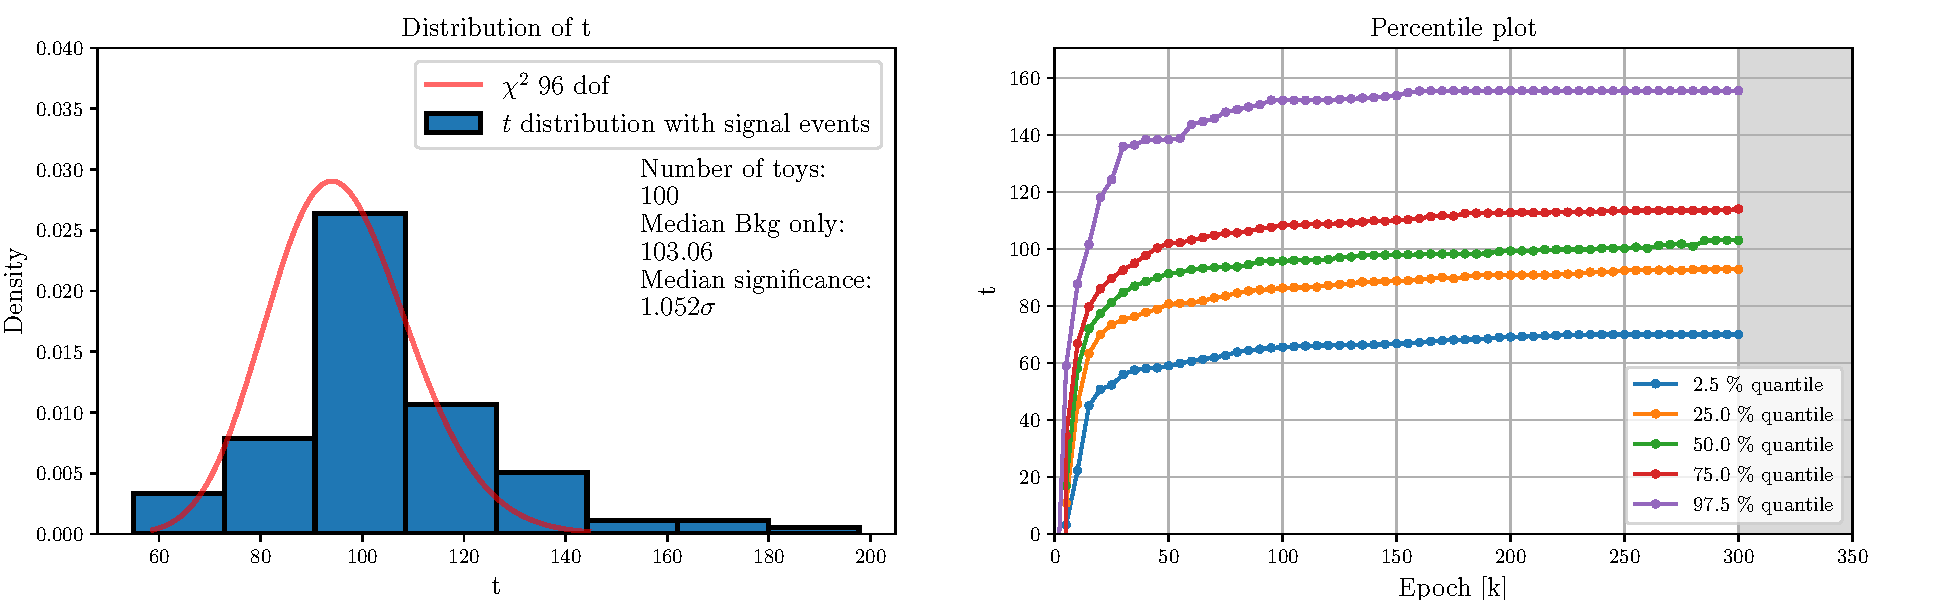
\includegraphics[width=1.0\textwidth]{Python/RESULTS/ref300000_bkg0_eft20000/data_ref300000_bkg0_eft20000_wclip2-45.pdf}
	\caption{Results for $N_\mathrm{ref}=300\si{k}$, $N_\mathrm{eft}=20\si{k}$, $W=2.45$.}
	\label{fig:REF300000_BKG0_EFT20000_WCLIP2.45}
\end{figure}
\vspace{-5mm}
\begin{figure}[H]
	\centering
	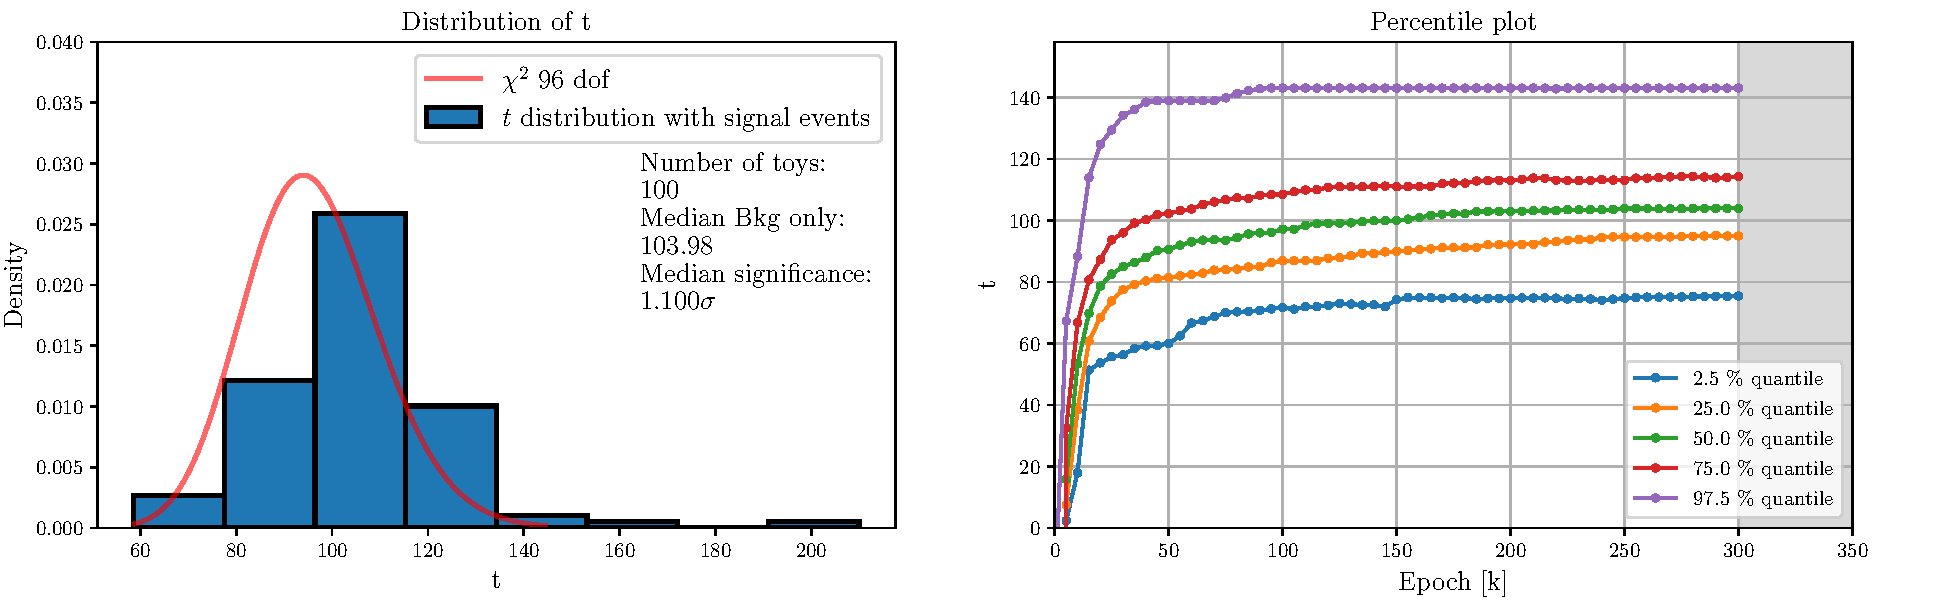
\includegraphics[width=1.0\textwidth]{Python/RESULTS/ref500000_bkg0_eft20000/data_ref500000_bkg0_eft20000_wclip2-55.pdf}
	\caption{Results for $N_\mathrm{ref}=500\si{k}$, $N_\mathrm{eft}=20\si{k}$, $W=2.55$.}
	\label{fig:REF500000_BKG0_EFT20000_WCLIP2.55}
\end{figure}




\subsection*{Observed significances}

\begin{table}[H]
	\centering
	\begin{tabular}{c c c c c c c}
		\toprule
		\multicolumn{4}{c}{\textbf{Zmumu-Zprime}}	&	\multicolumn{3}{c}{\textbf{EFT\_YW06}}	\\
		$N_\mathrm{ref}$	&	$N_\mathrm{bkg}$	&	$N_\mathrm{sig}$	&	$\sigma_\mathrm{med}$	&	$N_\mathrm{ref}$	&	$N_\mathrm{eft}$	&	$\sigma_\mathrm{med}$	\\
		\midrule
		100k	&	20k	&	40	&	3,873	&	100k	&	20k	&	1,556	\\
		200k	&	20k	&	40	&	4,025	&	200k	&	20k	&	1,216	\\
		300k	&	20k	&	40	&	3,766	&	300k	&	20k	&	1,052	\\
		500k	&	20k	&	40	&	3,721	&	500k	&	20k	&	1,100	\\
		1000k	&	20k	&	40	&	4,059	&	1000k	&	20k	&	2.016	\\
		\bottomrule		
	\end{tabular}
	\caption{Median significances observed at the end of training.}
	\label{tab:MED_SIG}
\end{table}

\begin{figure}[H]
	\centering
	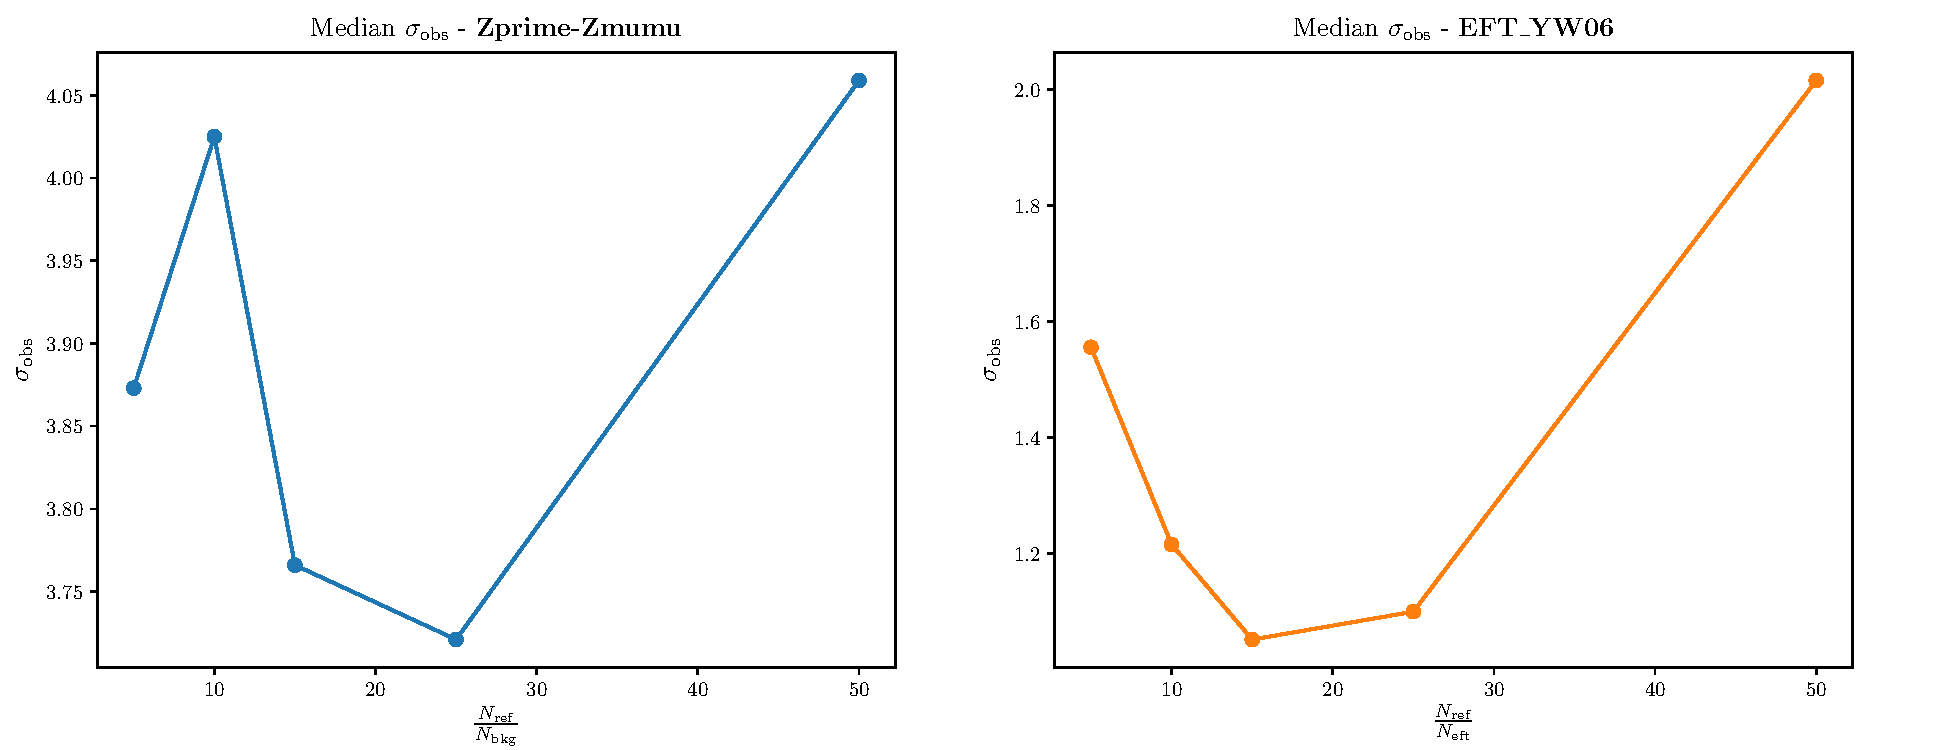
\includegraphics[width=1.0\textwidth]{Python/RESULTS/MED_SIG/med_sig_plot.pdf}
	\caption{Median $\sigma_\mathrm{obs}$ to varying of the ratio between $N_\mathrm{ref}$ and $N_\mathrm{data}$.}
	\label{fig:MED_SIG_CURVE}
\end{figure}

The trend of the median $\sigma_\mathrm{obs}$ gives us informations on what the network learns from the data fed to it. Higher values of $\sigma_\mathrm{obs}$ are obtained when the reference size is wide enough or small. A possible explanation can be given by highlighting two remarks:
\begin{itemize}
	\item When the reference size is small, the fluctuations in the data could be seen by the network as new physics signals. Therefore the significance increases on average.
	\item When the reference size is higher, the influence of the statistical fluctuations on the results is less relevant, but the differences between signal and background events are more pronunced. So the network has a more classification power after training and the significance becomes greater.
\end{itemize}
For a middle size of the reference none of these effects is relevant, so we find a minimum in $\sigma_\mathrm{obs}$ plot.

In general, the performances of the algorithm are much better in the case of the \textbf{Zmumu-Zprime} dataset respect to the corresponding value of the ideal significance. However, more operations can be done in order to enhance the power of the test statistic performed by the trained network and in the conclusion Chapter some of the possible improvements are stated along with the future development of this work.





\section{Training results: NN output analysis}
The final part of the analysis consits of studying the output $f(x)$ of the network. In the statistical foundation of the algorithm it was explained that $f(x)4$, when training is completed, approximates the log-likelihood ratio between the data distribution and the reference one. An interesting result arise when we plot $f(x)$ vs the invariant mass corresponding to every event $x$.

\begin{figure}[H]
	\centering
	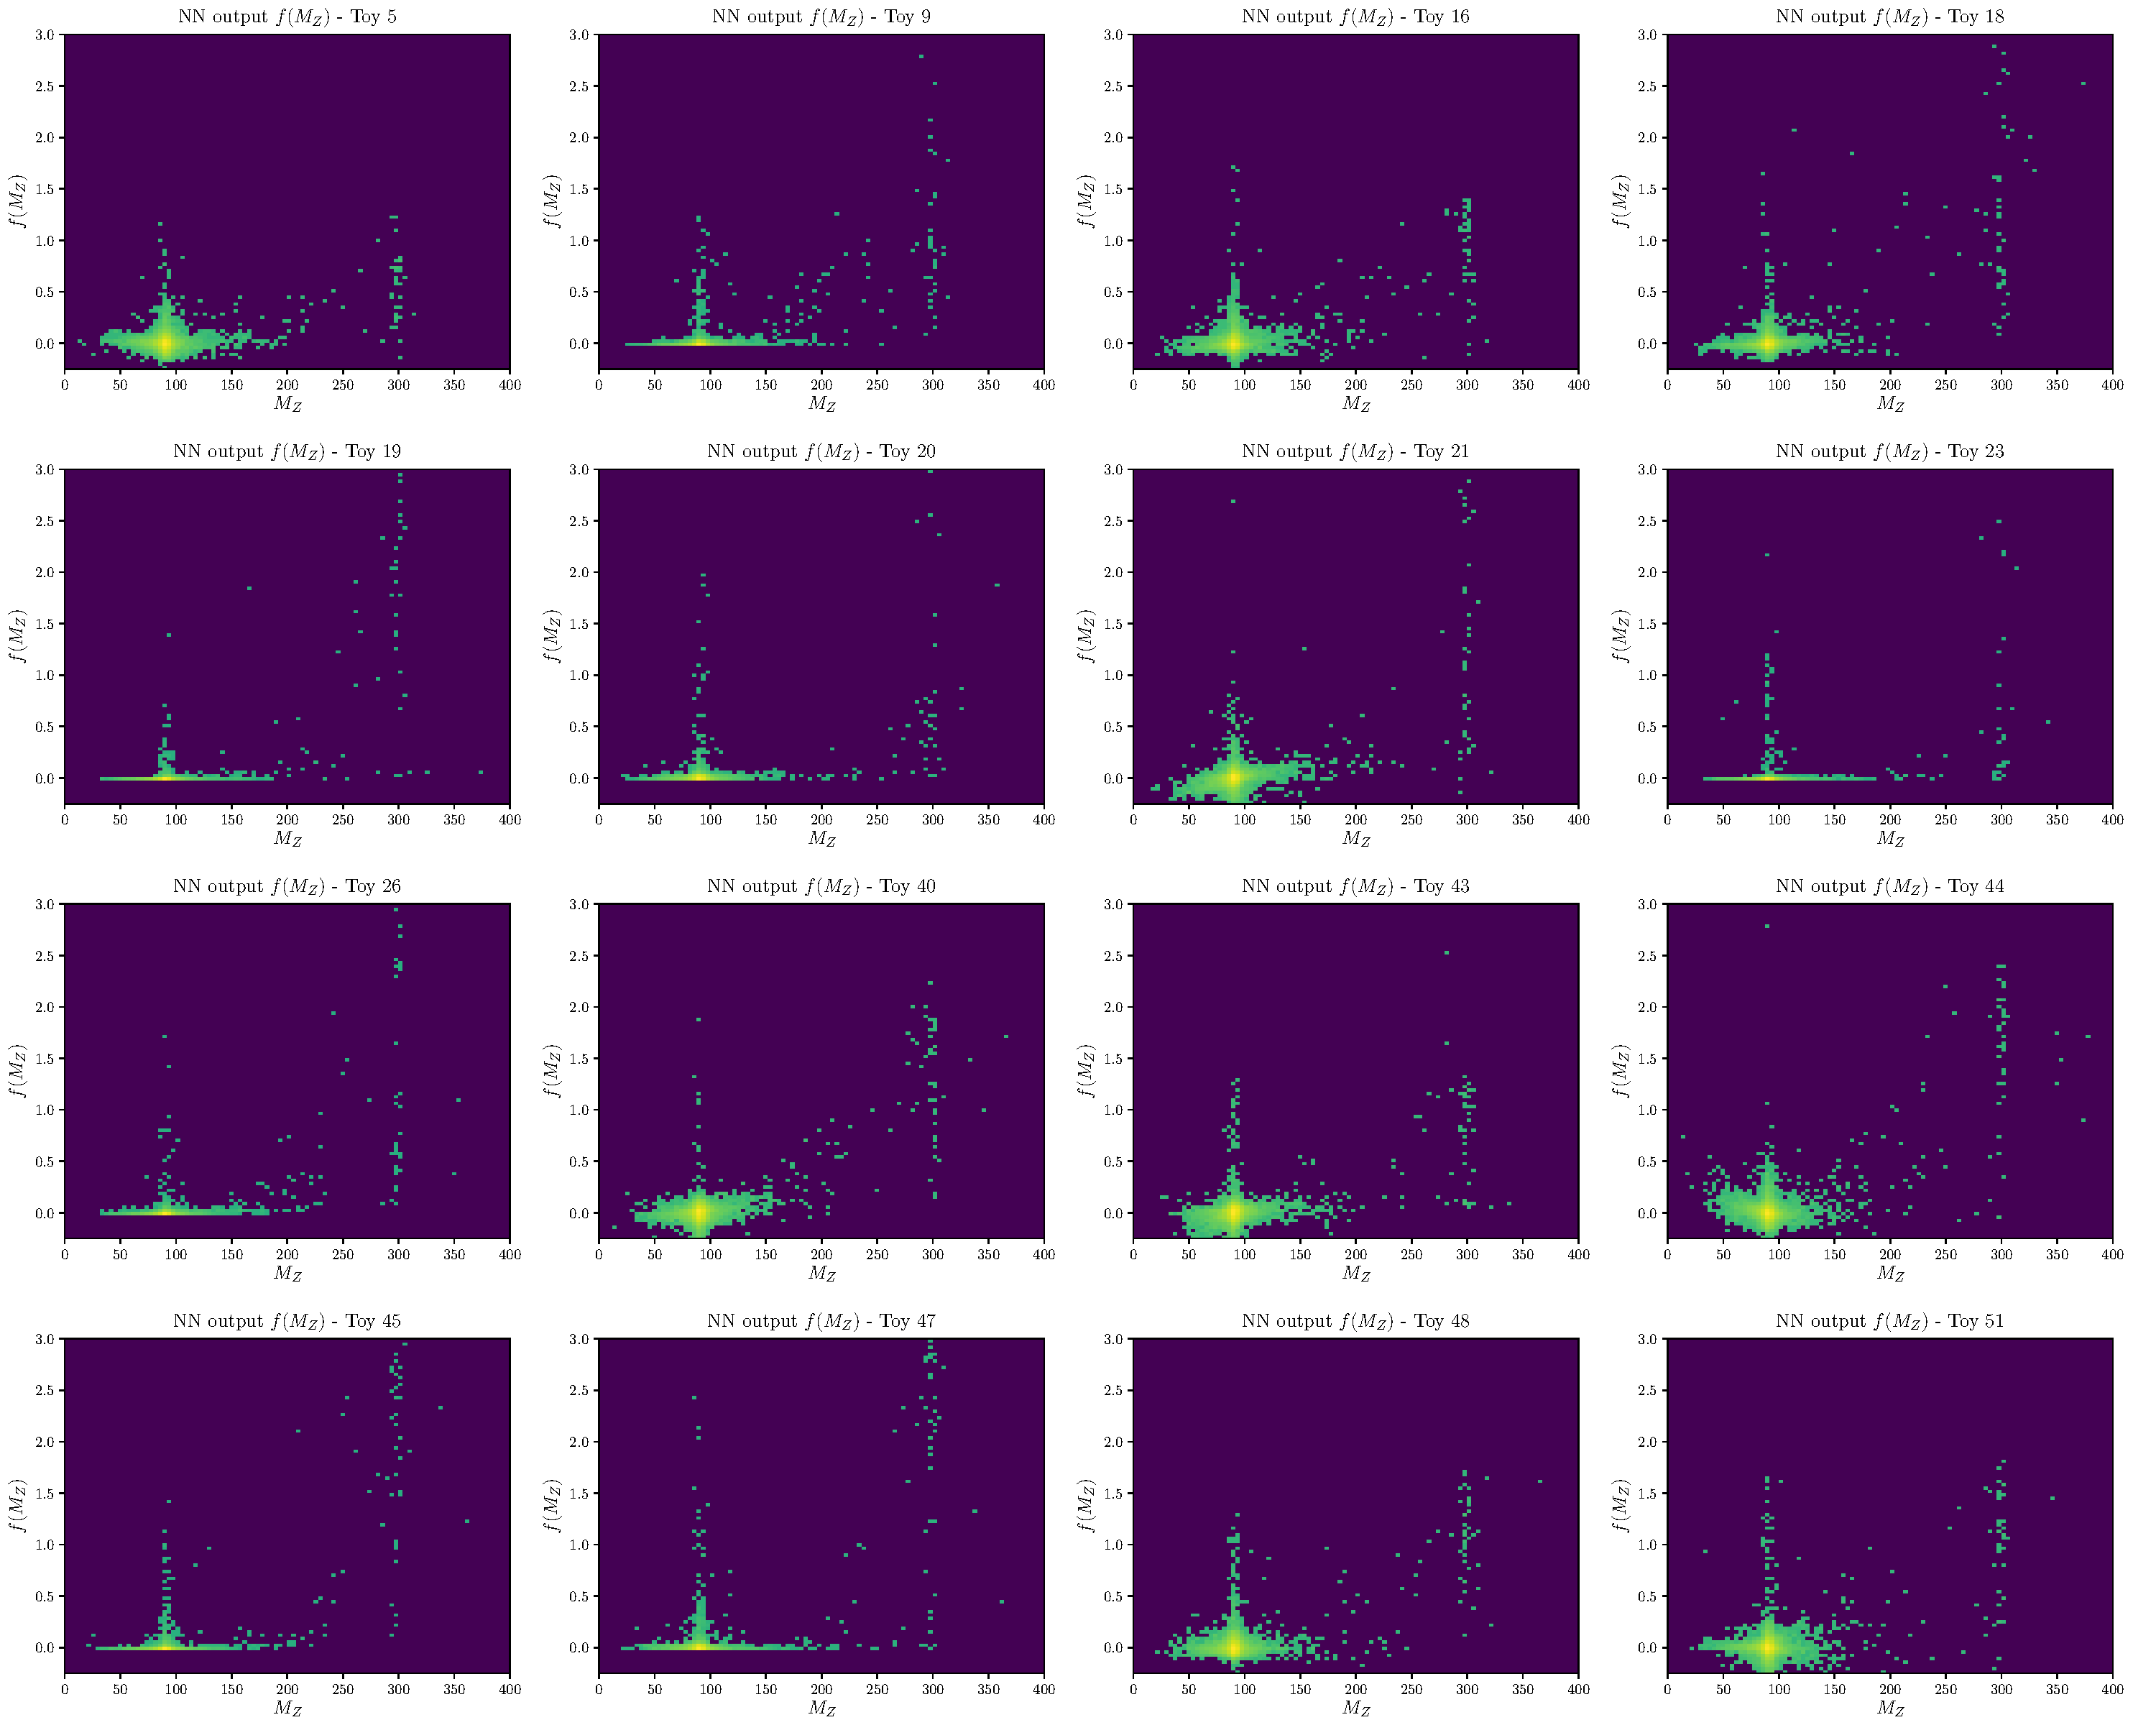
\includegraphics[width=1.0\textwidth]{Python/RESULTS/INV_MASS/f_plot.pdf}
	\caption{NN output $f(M_{Z})$ for different toys for \textbf{Zmumu-Zprime} with $N_\mathrm{ref}=1000\si{k}$, $N_\mathrm{bkg}=20\si{k}$, $N_\mathrm{sig}=40$, $W=2,7$.}
	\label{fig:F_PLOT}
\end{figure}


